\begin{figure}[!h] 
\centering 
\includegraphics[height=3in]{images/original/34cloudpirker1schulze10070aor}
%[width=.96\textwidth]
\caption{Cloud P1 Schulze 10070 & AOR}
\label{fig:34cloudpirker1schulze10070aor} 
\end{figure}

%SCT: sn = 10070 [Pa]  \307AORexp= 38.85\260, coeff. P. = 1
% \begin{figure}[htp]
%     \centering
%     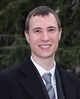
\includegraphics[width=.2\textwidth]{images/vitae/lbenvenuti}
%     \caption{OpenMP, MPI, MPI/OpenMP Hybrid runs of Box in a box testcase on 32
%     cores. The OpenMP-only run suffers from limited memory bandwidth in
%     memory-bound algorithms inside of the Modify section of the code. MPI-only has
%     low averaged runtimes for each section, but a very large Other timing, which
%     hints for a large amount of load-imbalance. Hybrid timings are a bit worse
%     on average, but because of better balancing, processes have lower wait times
%     inside of Other timing.}
% 	\label{fig:boxInBoxComparison}
